\documentclass[11pt,letterpaper,final] {article}

%%%%%%%%%%%%%%%%%%%%%%%%%%%%%%
% Packages
%%%%%%%%%%%%%%%%%%%%%%%%%%%%%%

	\usepackage[margin=1in]{geometry}
	\usepackage{amsmath}
	\usepackage{amsfonts}
	\usepackage{fancyhdr}
	\usepackage{graphicx}
	\usepackage{apacite}
	% \usepackage{tikz}
	% \usepackage{setspace}
	% \usepackage{multicol}
	% \usepackage[left]{lineno}

%%%%%%%%%%%%%%%%%%%%%%%%%%%%%%
% Page styling
%%%%%%%%%%%%%%%%%%%%%%%%%%%%%%
	
	%%%%%%%%%%%%%%%%%%%%
	% Headers and footers
	%%%%%%%%%%%%%%%%%%%%
	
	\pagestyle{fancy}
	\renewcommand{\headrulewidth}{0pt}
	\fancyhead{}
	\fancyfoot{}
	\rhead{Page \thepage}
	\lhead{Test \#12}
	
	%%%%%%%%%%%%%%%%%%%%
	% Graphics path
	%%%%%%%%%%%%%%%%%%%%
	
	\graphicspath{{./assets/}}
	
	%%%%%%%%%%%%%%%%%%%%
	% Frontmatter
	%%%%%%%%%%%%%%%%%%%%
	
	% \title{The Title}
	% \author{The Author}
	% \date{\today}
	
	

%%%%%%%%%%%%%%%%%%%%%%%%%%%%%%
% Custom definitions
%%%%%%%%%%%%%%%%%%%%%%%%%%%%%%
	% Easy scientific notation
	\newcommand{\e}[1]{\ensuremath{\times 10^{#1}}}
	
	% Textual subscripts
	\newcommand{\sub}[1]{\ensuremath{_{\text{#1}}}}
	
	% Textual superscripts
	\newcommand{\super}[1]{\ensuremath{^{\text{#1}}}}

\begin{document}

% \linenumbers
% \maketitle

\paragraph{Question 01.} Granuloma, an aggregation of various immune cells, is typically considered a hallmark of tuberculosis infection and represents a crucial step in the control and eradication of mycobacterial infection. Yet, the formation of such requires the contribution and interaction of many types of immune cells.

Specifically, research has indicated that activation of $\alpha\beta$ T cell receptor-expressing CD4\super{+} T cells is a crucial step in the formation of these granulomas (Saunders, Frank, Orme, \& Cooper, 2002). However, this step, although necessary, is not alone sufficient for their formation: indeed, $\alpha\beta$ TcR-expressing CD8\super{+} T cells, $\gamma\delta$ TcR-expressing T cells, and CD1-restricted CD4\super{-}CD8\super{-} T cells have all been implicated additionally (Mogues, Goodrich, Ryan, LaCourse, \& North, 2001). Additional immune cell types are then recruited, summarized below in Figure \ref{fig:00}.

\begin{figure}[htp]
  \centering
    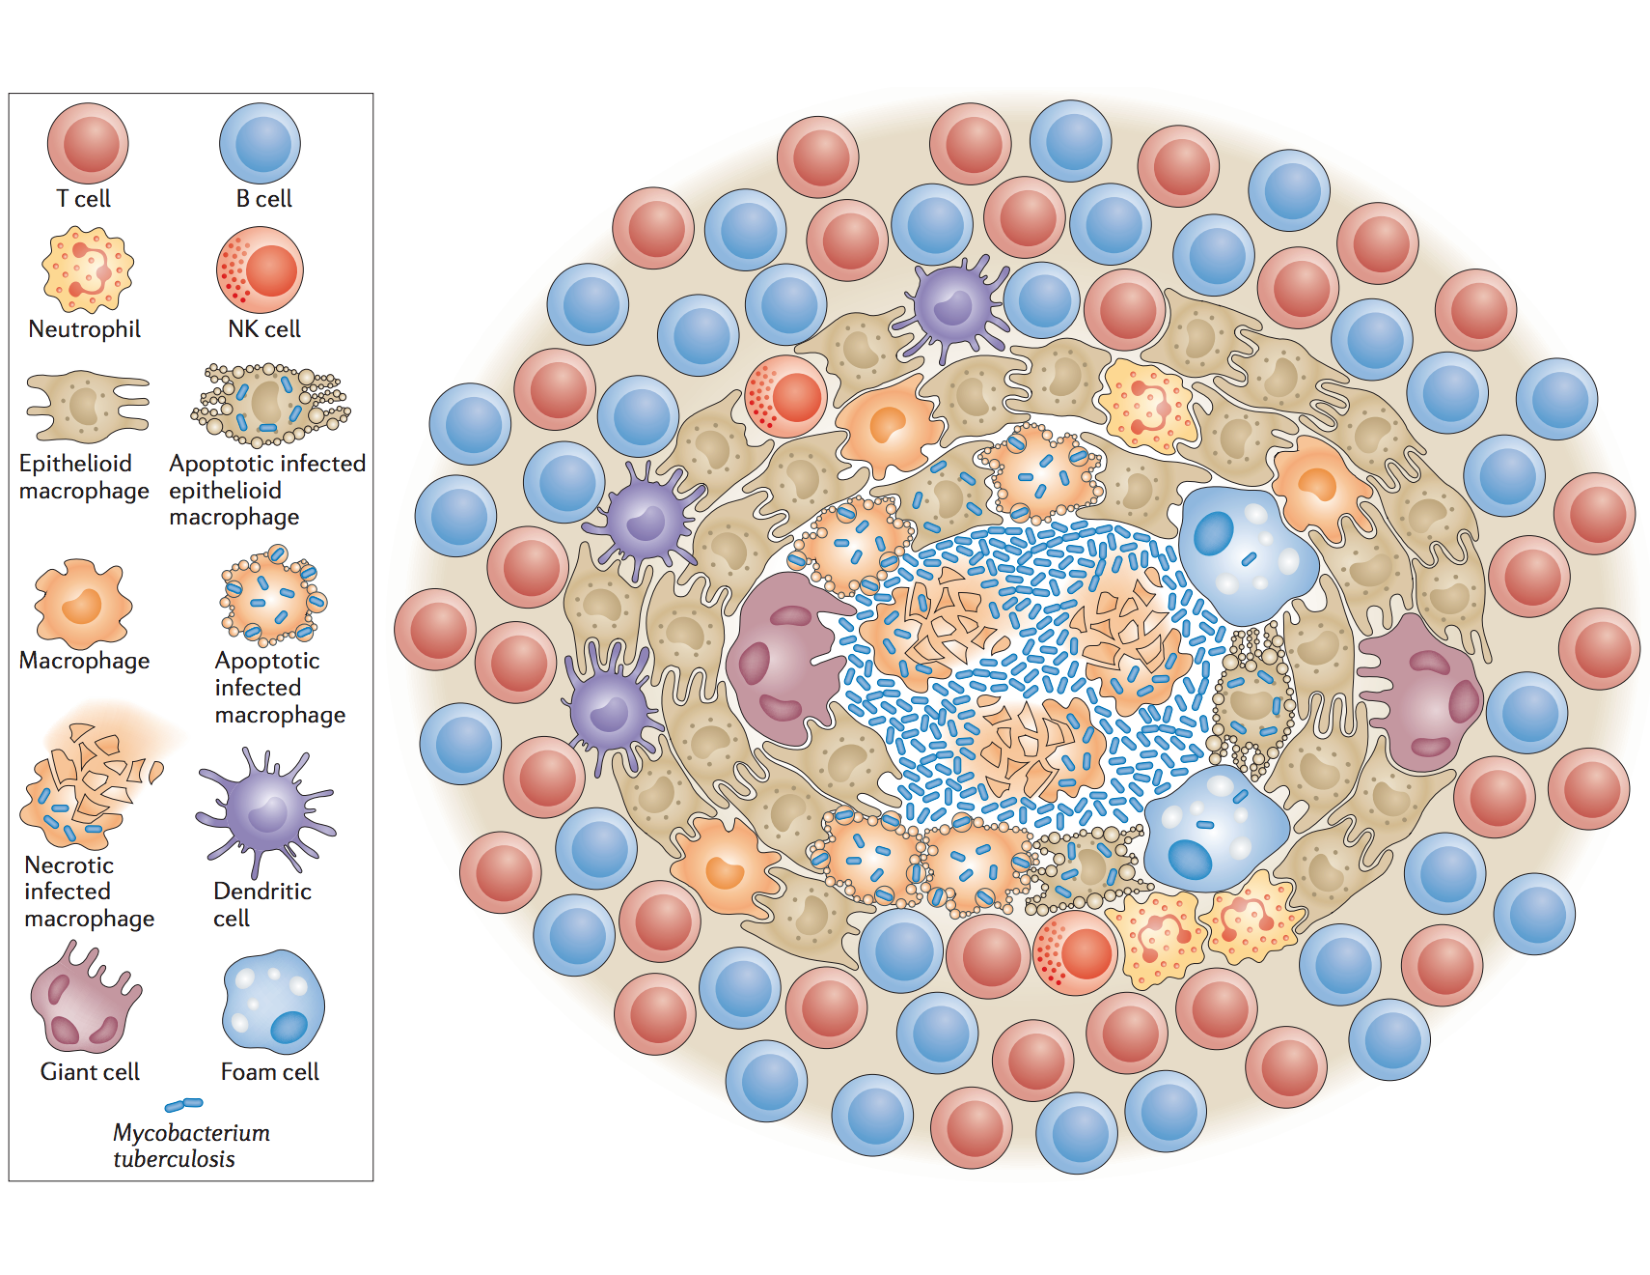
\includegraphics[width=0.65\textwidth]{granuloma}
	\caption{Structure of tuberculosis granuloma. Excerpted from Ramakrishnan (2012).}
	\label{fig:00}
\end{figure}

In response to tuberculosis challenge, we see an initial and rapid migration of macrophages to the sire of infection. These cells phagocytose the contents of other dying (infected) macrophages and themselves become then infected. Recent work has additionally described the expression of CCL19 and CCL21, chemokine ligands characteristically expressed in the lymphoid organs, in the lungs. Expression of MMP9 has been shown to further recruit macrophages to the site of infection.

At some delay, effector T cells are recruited to the site of infection, and this correlates with the control of infection (Cooper, 2009).  This lag may be attributable to the action of T\sub{reg} cells, present at the site of granuloma, that counteract host mechanisms to induce T\sub{H}17 cells that then promote the recruitment of T\sub{H}1 cells (Khader et al., 2007). 

\paragraph{Question 02.} Systemic lupus erythematosus (SLE) is an autoimmune disorder in which autoantibody production results in chronic inflammatory damage to multiple host organ systems \cite{Dong:2011}. Emerging evidence suggests that populations of T\sub{H} cells produce IgG class-switched autoantibodies that contribute to the pathogenesis of lupus \cite{Datta:2005}. In such a model, stylized in Figure \ref{fig:01}, we see inappropriate T\sub{H} cell activation following recognition by B cells (or other antigen presenting cells) of autoantigens and subsequent loading of those peptide epitopes onto MHCII molecules.

\begin{figure}[htp]
  \centering
    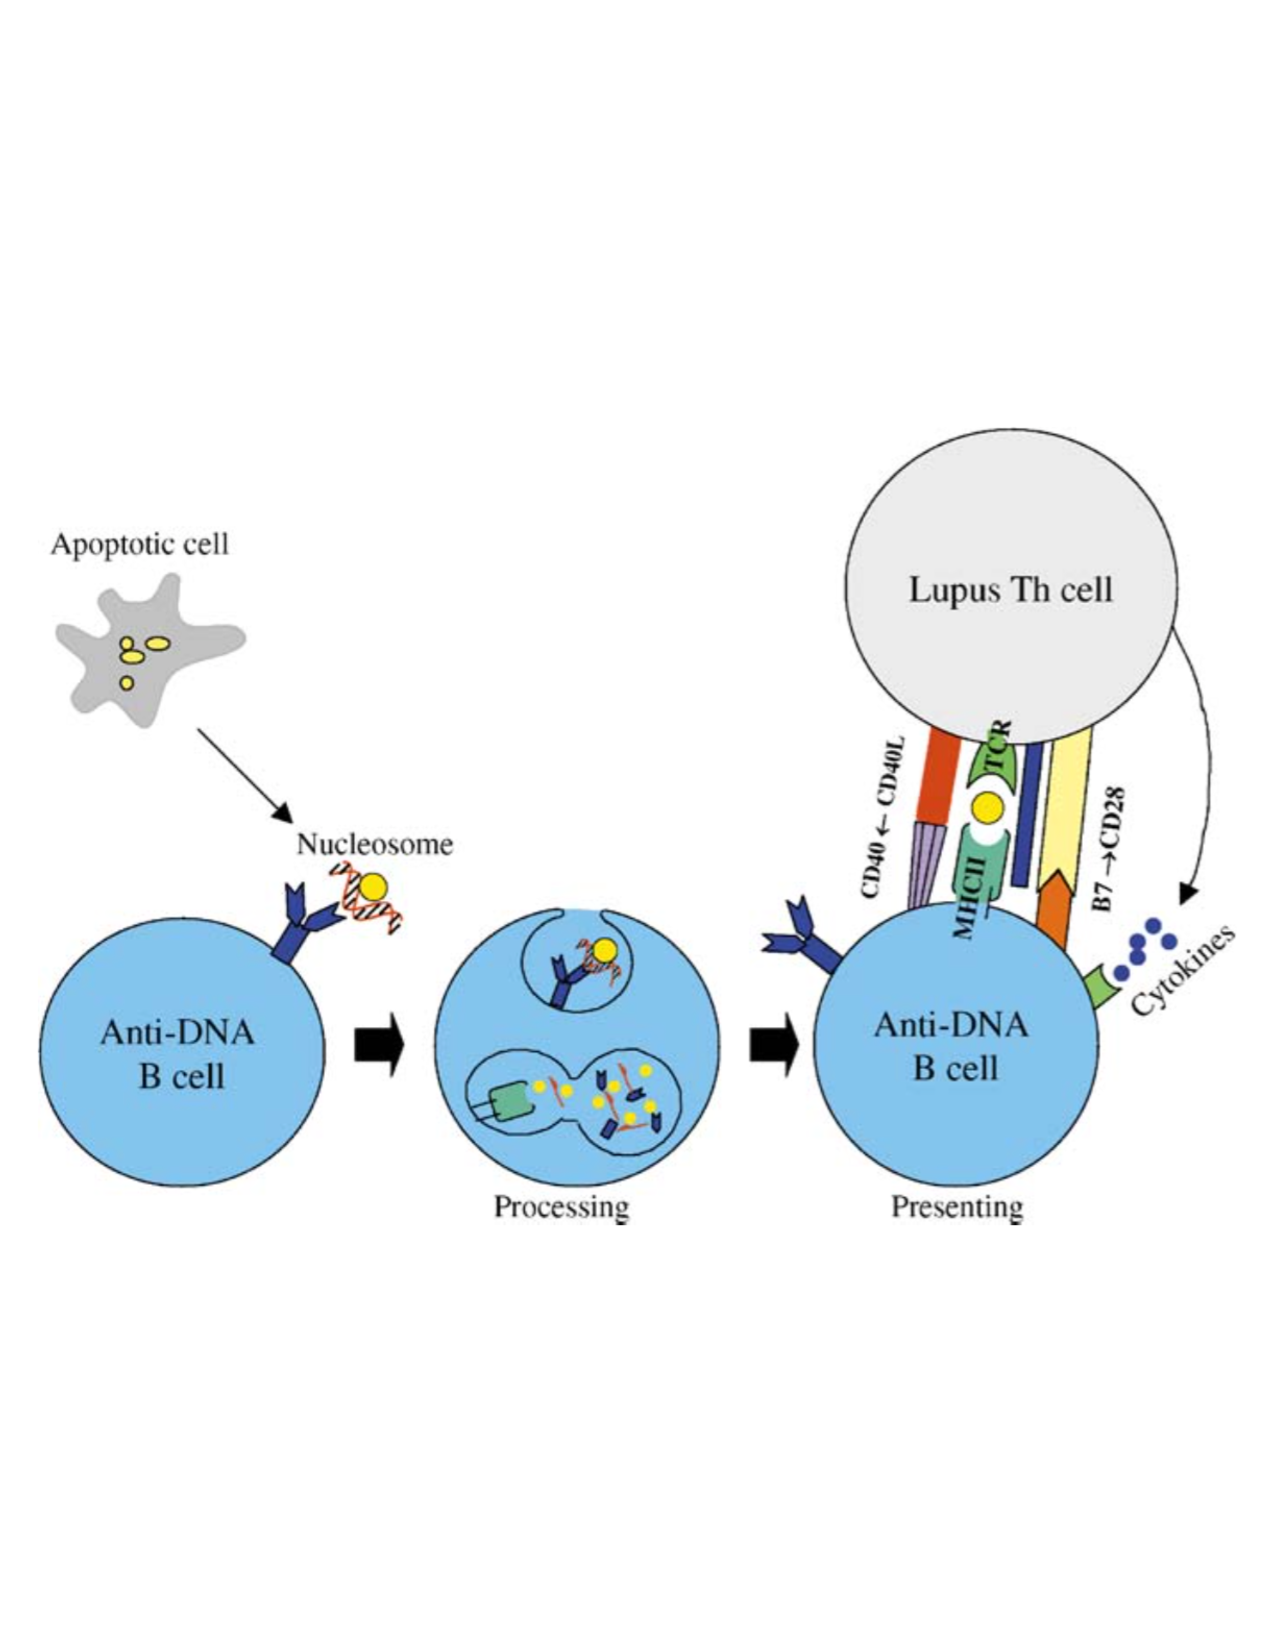
\includegraphics[width=0.65\textwidth]{sensitization}
	\caption{Stylized representation of inappropriate T\sub{H} cell activation following B cell sensitization to autoantigens. Taken from Datta, Zhang, and Xu (2005).}
	\label{fig:01}
\end{figure}

What is unclear, however, is the role that T regulatory cells may play in the pathogenesis of this disorder. Specifically, the primary responsibility of regulatory T (Treg) cells is to shut down the host's immune response following successful clearance of an invading pathogen or other immune challenge \cite{Shevach:2000}. On this basis, one might suspect some deregulation of Treg populations as contributing to the pathogenesis of SLE: that is, lupus is a chronic disorder characterized by sporadic attack by immune cells of healthy host organs and tissues.

Importantly, we also see that the progression of SLE is often sporadic and unpredictable, with periods of alternating illness and remission. As such, we might hypothesize that these periods of remission are influenced by the modulation of Treg cell populations that serve to delete autoreactive T cells in the thymus.

Indeed, in recent literature we see support for this hypothesis: work by both Mudd, Teague, and Farris and Robak, et al. have shown evidence for decreased numbers or impaired function of CD4\super{+}Foxp3\super{+}CD25\super{+} regulatory T cells (2006; 1999). More recent work has further shown that, likewise, the CD27\super{+}CD45RA\super{−} $\gamma\delta$ T cell population of SLE patients is significantly decreased (Xiaoyan et al., 2011).

Given this preliminary evidence correlating decreased Treg cell populations with SLE patients, to test any cause-and-effect relationship between the two, we may utilize a DEREG (DEpletion of REGulatory T cells) murine model in which CD4\super{+}Foxp3\super{+} Tregs can be rapidly and nearly completely ($\sim$95\% efficiency) depleted upon administration of diphtheria toxin. Mice of this lineage could be cross-bred with, for instance, NZB/W F1 mice which develop severe lupus-like phenotypes comparable to those of SLE patients (Theofilopoulos \& Dixon, 1985). (Alternately, MRL/\textit{lpr} or BXSB/\textit{Yaa} mouse models could be utilized if the presence of autoantibodies against RNA-containing complexes is important.) In any event, this cross would result in a mouse line manifesting spontaneous SLE symptoms and with Treg cell populations that can be readily and almost completely depleted.

Our research program might then begin by evaluating up- or downregulation of Treg populations at varying time points in the development and onset of SLE-like symptoms in our mice to first establish that they manifest a similar response with respect to their Treg cell populations as has been observed in human SLE patients. In the event that this is not observed, a different animal model of SLE may have to be selected that can reasonably be thought to recapitulate the human Treg cell response to SLE with greater fidelity.

Following this, we could, keeping all else equal, deplete the mouse Treg population, predicting a worsening of the SLE phenotype, or the onset of illness if in remission when the cell population is depleted. Conversely, after allowing this population to rebound, we would expect the SLE phenotype to be ameliorated.

Additionally, we could employ an induced lupus model (e.g., pristane-induced), whereby we could attempt to induce an SLE phenotype with normal and depleted Treg populations (a more severe phenotype would be expected in the Treg-depleted population).

\paragraph{Question 05.} Immunosenescence refers to the general decline of immune functioning with age of the individual, reflected by increased susceptibility to infectious disease, increased prevalence of cancer, and affliction with other similarly detrimental conditions. Yet, the precise causes of this are not fully known. Three theories of immunosenescence exist: that with age, the ability to distinguish between foreign and self diminishes; that the immune system with age becomes unable to adequately defend from invading pathogens; and that with ageing comes the disruption of various components of immune processes.

Regardless, with age we see certain definite changes to various components of the innate and adaptive immune responses. For instance, skin and other mucosal barriers, the first line of defense against pathogens, see reductions in rates of cellular replacement. The skin loses its population of Langerhans cells. However, a global decrease in the number of dendritic cells is not seen. Rather, only specific populations appear to be depleted, such as Langerhans cells and plasmacytoid dendritic cells (Grewe, 2001; Jing et al., 2009). Yet, although dendritic cell populations are largely left undiminished, we do observe a decrease in pattern recognition receptor function with age (Kumar, Kawai, \& Akira, 2009). Some evidence additionally shows that migration is negatively affected via the pi3k pathway.

With respect to adaptive immunity, with age comes a decreased ability of hematopoeitic stem cells to proliferate (Lansdorp et al., 1994). Along with this, there is a decrease in B cell diversity (seen as a decrease of naive B cells and increase in memory B cells) (Gibson et al., 2009). Further, a general decrease in high-affinity antibody production is observed, although the mechanisms of somatic hypermutation are preserved (Roukens et al., 2011; Dunn-Walters, Manerjee, \& Mehr, 2003). As with B cells, a decrease in naive T cells is observed with age, and is accompanied by a decrease in the absolute number of T cells (Koch et al., 2008). This and other changes to T cell populations is generally associated with increased prevalence of age-related disease (Olsson et al., 2000).

Finally, with age we see the emergence of a chronic, low-grade inflammatory state, although this may be somewhat inhibited by the circulation of anti-inflammatory cytokines. Specifically, generally an increase in IL-1, IL-2, IL-6, IL-8, IL-10, IL-12, TNF-$\alpha$, and IFN-$\gamma$ are all upregulated. These changes are often associated with age-related disease such as atherosclerosis, Alzheimer's, and osteoperosis.

\paragraph{Question 07.} Rabies is a viral infection transmitted primarily through the saliva of an infected host, often following a bite. (However, transmission through organ transplantation has been observed, albeit rarely (e.g., Javadi, Fayaz, Mirdehghan, \& Ainollahi, 1996).) Although human-to-human transmission is quite rare, canines remain an important reservoir of the virus worldwide, and particularly in developing countries (Taylor, 2013). Indeed, we may see as much in Figure \ref{fig:02}. Yet, despite the prevalence of this disease in much of the world and the high rate of mortality if untreated (approaching 100\%), due largely to lack of infrastructure, it is believed that the true number of annual cases remains underreported and this lack of accurate data has been identified as a primary obstacle in making rabies eradication a public priority (Fooks et al., 2014).

\begin{figure}[htp]
  \centering
    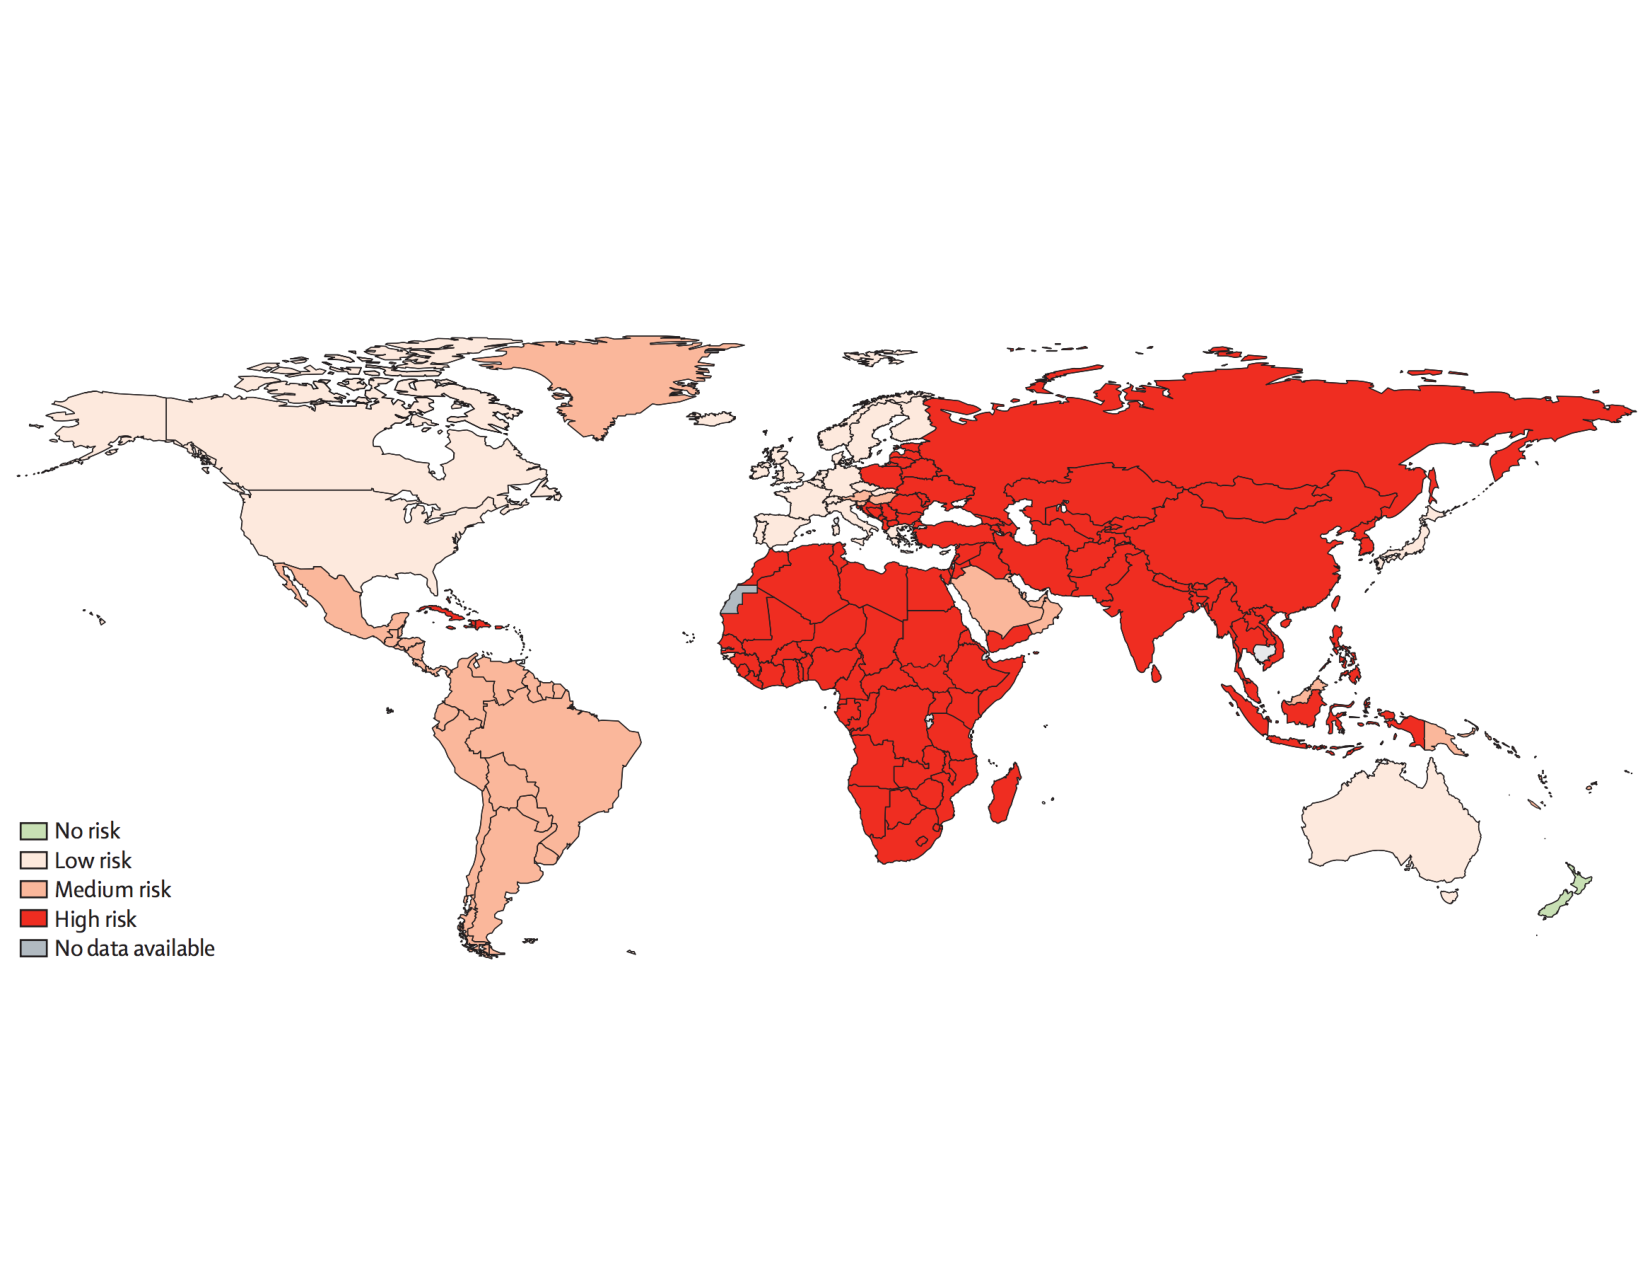
\includegraphics[width=0.65\textwidth]{rabies}
	\caption{Relative risk of contracting rabies worldwide. Data taken from WHO. Figure excerpted from Fooks et al. (2014).}
	\label{fig:02}
\end{figure}

With respect to humans, transmission of rabies from canine bite accounts for up to 99\% of all new cases and, as such, control and elimination of infected canine populations is a crucial step in the worldwide eradication of the disease. However, bats have also been identified as a natural reservoir of for lyssaviruses. (An exception to this being for  MOKV and Ikoma lyssavirus, for which no natural reservoir has yet been identified (Banyard et al., 2013).) Moreover, most mammals have been shown capable of being infected with RABV (the remaining lyssaviruses are typically only found in bats), although few of these species have demonstrated a capability to act as long-term reservoirs for the virus (Badrane \& Tordo, 2001).

On this understanding, we see the potential for critical gaps in rabies surveillance. Specifically, it is thought that RABV evolved initially in species of the order Chiroptera (i.e., bats) and then species-hopped to other (largely carniverous) mammals. This would indicate the possibility not only of other lyssaviruses doing the same, even given the successful global eradication of RABV, but also the potential for the establishment of other natural reservoirs not previously observed, given an appropriate selective pressure.

As such, for the truly successful eradication of rabies virus, we must see: (1) adequate political will and financial investment in healthcare infrastructure and reporting in developing nations; (2) the active control of rabies virus-infected canine populations at a global scale; (3) ongoing surveillance of other carnivorous mammalian species for their establishment as novel natural reservoirs; and (4) eradication of the virus in wild bat populations to prevent its reintroduction into terrestrial mammals. Furthermore, identification of the natural reservoirs for the MOKV and Ikoma lyssaviruses should be seen as crucial, for clearly, although we have identified the two primary species (bats and dogs) responsible for the maintenance and transmission of rabies virus, our inability to claim this knowledge for all 12 distinct lyssavirus virus species (by International Committee on Taxonomy of Viruses delineation) indicates that there exist populations wherein the virus is circulating which we have no hope of surveilling or controlling. Until such point that we have identified all natural reservoirs of lyssaviruses, there remains considerable potential for the adaptation of these viruses to novel mammalian hosts, further hampering any attempts to control their spread.

\paragraph{Question 08.} There exist several distinct mechanisms by which organisms may evolve in response to positive and negative selective pressures: primarily, horizontal gene transfer; \textit{de novo} mutation (indels; SNPs); and genetic reassortment and recombination.

As seen in Figure \ref{fig:03}, small RNA viruses and ssDNA viruses (both with relatively small genomes) are the primary drivers of evolution-by-\textit{de novo} mutation. Although (as shown below) far from their exclusive evolutionary mechanism, their high rate of replication and error-prone RNA-dependent RNA polymerase allow for relatively high rates of random mutation without catastrophic consequences to the overall fitness of the whole viral population within the host. (I.e., although many mutants may be non-viable, the rate of replication is high enough and the error rate of the RDRP high, but nonetheless low enough that enough virions remain viable to allow for sustained proliferation.) In higher-order organisms (e.g., eukaryotes), the rate of \textit{de novo} mutation remains low, largely due to the proofreading mechanisms that exist to correct for errors in genome replication.

\begin{figure}[htp]
  \centering
    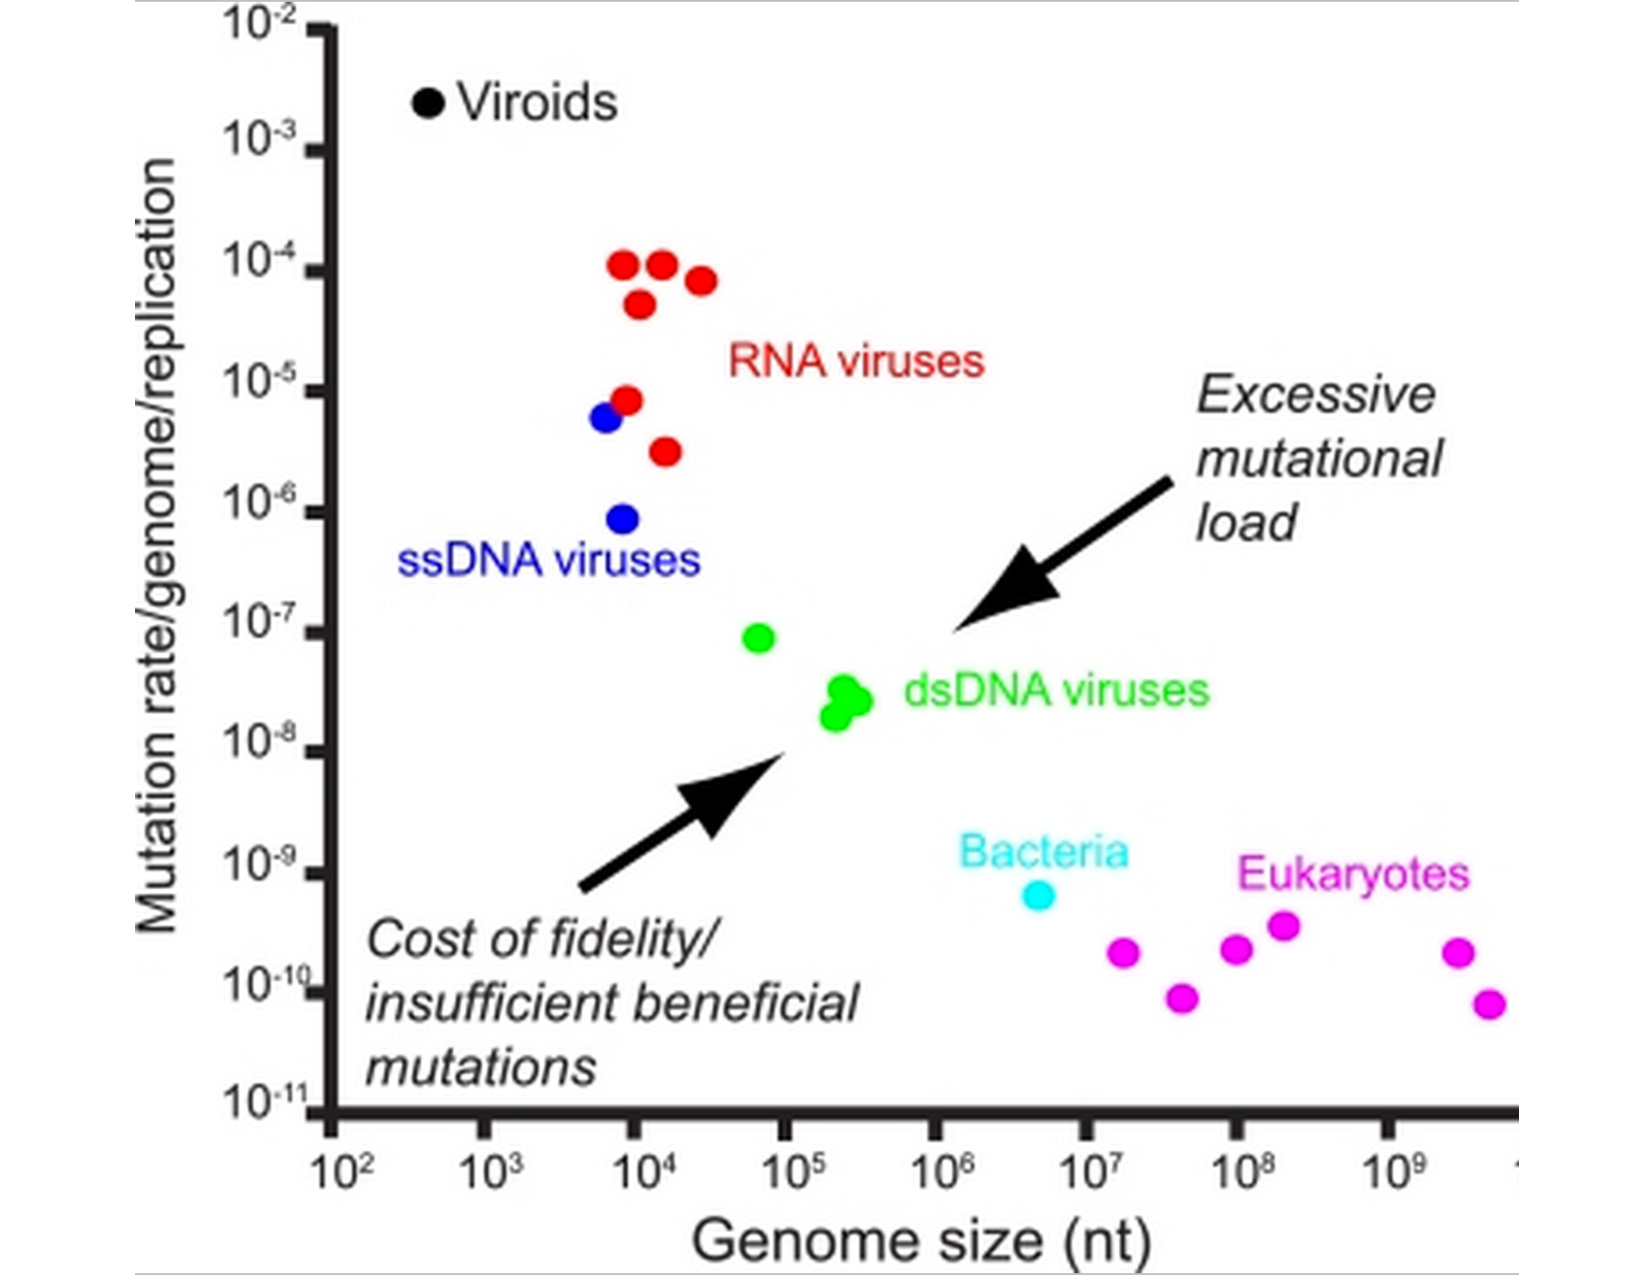
\includegraphics[width=0.65\textwidth]{mutation}
	\caption{Mutation rate versus genome size. Excerpted from Holmes (2011).}
	\label{fig:03}
\end{figure}

Among viruses, we see that this strategy is employed quite successfully, primarily with the goal of immune evasion. Influenza, for instance, is highly antigenically variable with respect to its HA and NA surface proteins: the high rate of mutation on these regions (typically the targets of annual flu vaccines) allows the virus to persist easily despite concerted annual vaccination and prevention efforts. Likewise, among, for instance, parasites such as \textit{P. falciparum} we see a similar evolutionary mechanism employed in the evolution of resistance to quinine and chloroquinine, via mutations to the \textit{pfcrt} allele (Valderramos et al., 2010).

Alternately, many bacteria, such as \textit{V. cholera}, will employ horizontal gene transfer systems. In the case of cholera, we observe horizontal transfer of genes is mediated by a type VI secretion system. In this way, the bacteria respond to inter-serogroup competition and external environmental pressures by the direct cell-to-cell exchange of genetic material (Unterweger et al., 2013).

With respect to genetic reassortment and recombination, we see these strategies broadly employed by diverse pathogens. Returning to influenza, having a segmented genome, multiple strains co-infecting a single host have the capability to swap gene segments with one another during replication to produce chimeric progeny, often enabling host species hopping of strains after, for example, acquiring genes encoding for receptor binding sites for a species to which the strain previously lacked.

\paragraph{Question 09.} Endogenous retroviruses represent genetic segments integrated into the germ line from exogenous infectious retroviruses and represent between 4 and 5\% of the human genome (Dewannieux \& Heidmann, 2013; Lander et al., 2001). Historically, endogenous retroviruses have been suspected in the development of cancers by a variety of mechanisms, summarized in Figure \ref{fig:04} (Weiss, 2006).

\begin{figure}[htp]
  \centering
    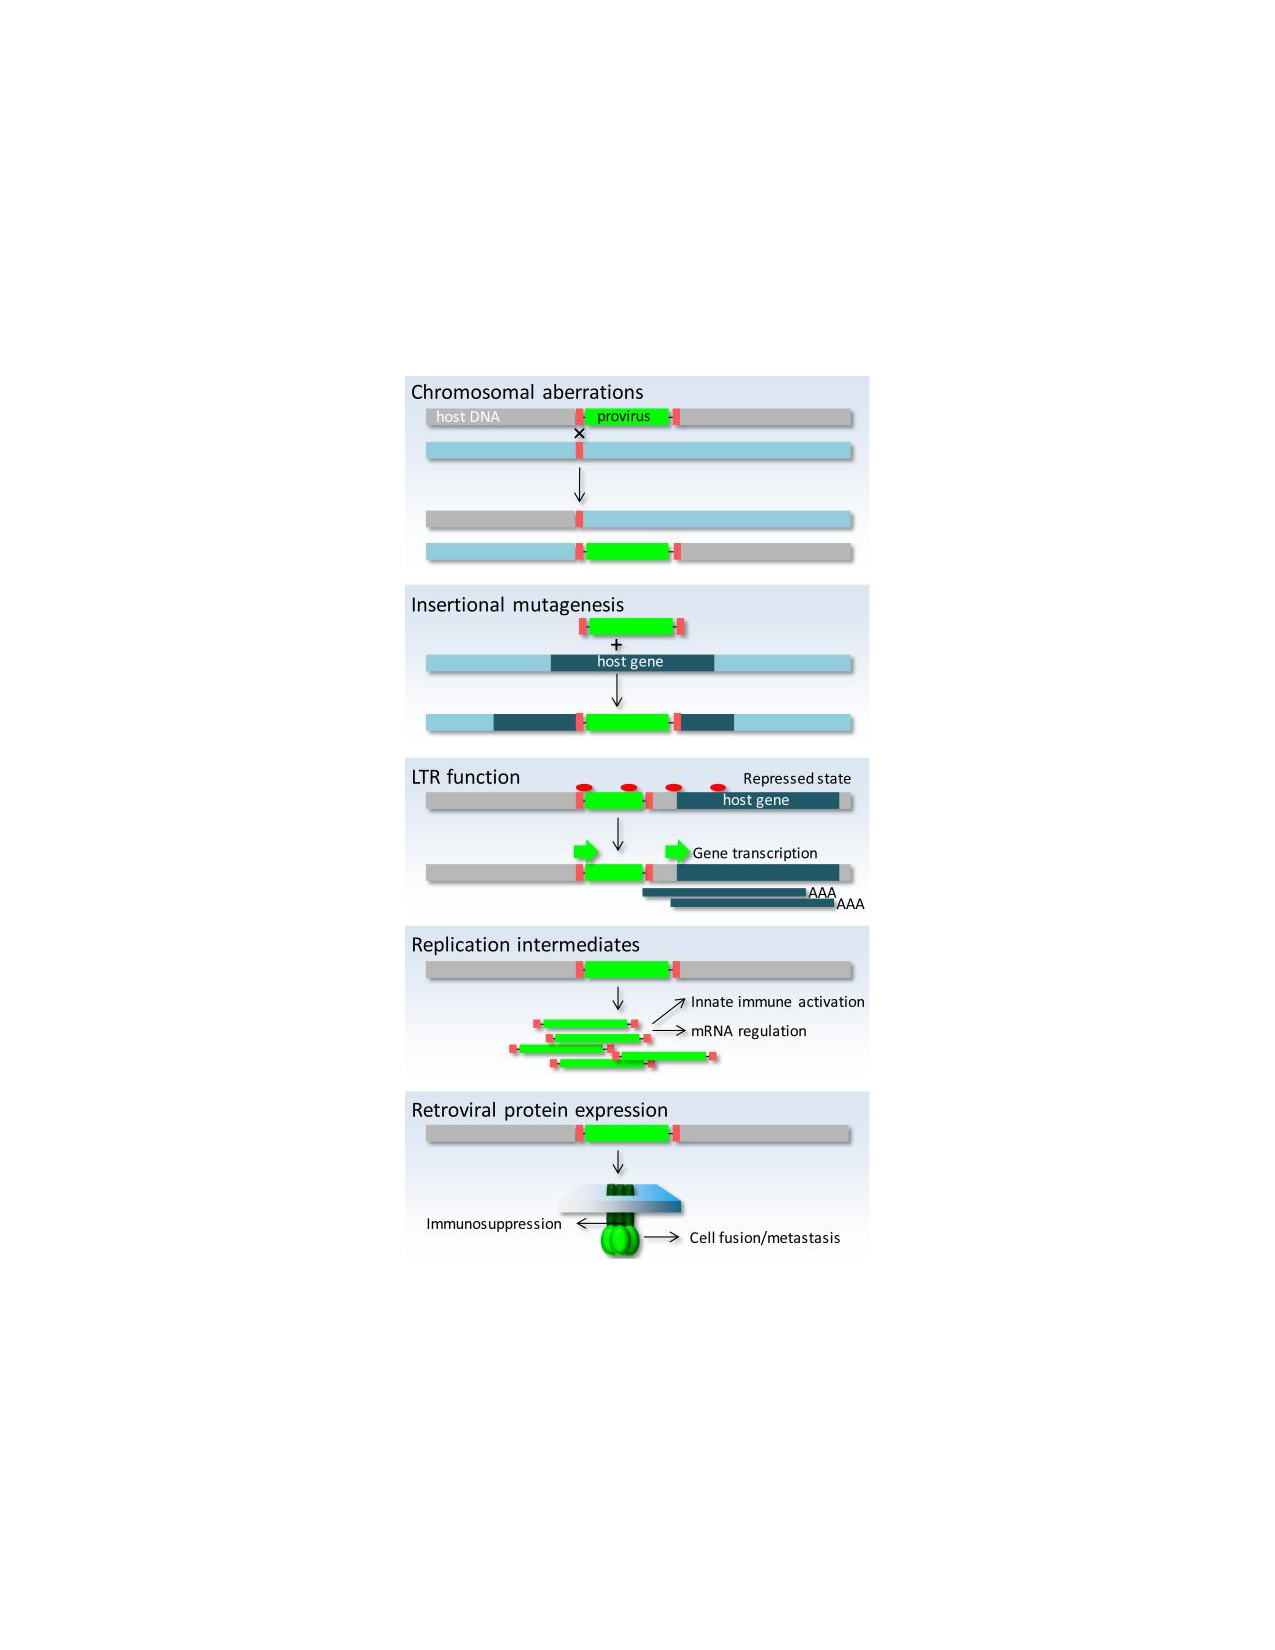
\includegraphics[width=0.65\textwidth]{retrovirus}
	\caption{Potential mechanisms of ERV-mediated transformation. Excerpted from Kassiotis (2014).}
	\label{fig:04}
\end{figure}

Tumor promotion by insertional mutagenesis was an initial suspect given research implicating xenotropic murine leukemia virus-related virus (XMRV) as a causative agent in prostate cancers (reviewed in Bhardwaji \& Coffin, 2014). Much of this resulted from a finding of MLV sequences among prostate tumor RNA, followed by successful isolation of a virus capable of infecting human prostate cancer cells and other common human cell lines. Ultimately, however, these initial studies were disproven and shown to be the result of contaminated samples rather than a genuine link between ERVs and oncogenesis.

Although exogenous human retroviruses capable of oncogenesis (e.g., human T-lymphotrophic virus 1) have been discovered, to date, no HERV provirus capable of producing an infectious retrovirus has been identified; however, infectious recombinants are capable of being generated (Kassiotis, 2014; Ruprecht et al., 2008).

Yet, many of these ERVs do still contain open reading frames that produce individual retroviral proteins. A small number of these proteins, such as Rec and Np9 (alternative splicing products of the HERV-K(HML2) \textit{env} gene), have been implicated in tumorigenesis (Ruprecht et al., 2008); however, proposed direct mechanisms of ERV protein-mediated oncogenesis remain few.

Further, there is potential for the noncoding RNA ERV transcripts and the ERV LTRs present in the genome to impact host genomic function (Jern \& Coffin, 2008). For example, polypyrimidine tract-binding protein (PTB)-associated splicing factor (PSF), a repressor of various proto-oncogenes, is known to bind to noncoding RNA, and its activity negatively regulated thereby. Specifically, it has been shown to bind to RNA transcripts from a HERV-K11 provirus (Li et al., 2009). As such, it is possible that ERVs may indirectly contribute to oncogenesis by inhibiting inhibitors of proto-oncogenes.

However, despite these putative mechanisms of ERV-mediated oncogenesis, direct and compelling evidence of causation remains elusive. Certainly, it is not a stretch to infer how these might be implicated in the onset of various cancers, yet without direct and well-controlled experimental data, a causal link cannot be established.

%%%%%%%%%%%%%%%%%%%%
%% REFERENCES
%%%%%%%%%%%%%%%%%%%%

\clearpage
\bibliographystyle{apacite}
\bibliography{references}

\end{document}